%        1         2         3         4         5         6         7         8         9         0         1         2
%23456789012345678901234567890123456789012345678901234567890123456789012345678901234567890123456789012345678901234567890
\documentclass[12pt]{MIA-USA}

\usepackage{layout}
\usepackage{subcaption}
\usepackage{paralist}
\usepackage{breakcites}
\usepackage{pgfgantt}
\usepackage{pdflscape}

%% Semana del 16 de junio ¡ANTEPROYECTO! 12 clases
% Cada trabajo vale lo mismo que el anterior. 16%
% 

% Trabajos, aproximadamente cada dos semanas.
% Problema y justificación [Título] (13 de marzo)
% Objetivos [General y espécificos (No más de 4)] (3 de abril)
%   * Cada objetivo espécifico se debe soportar por un capítulo en el proyecto.
% Estado del arte (17 de abril)
% Metodología (8 de mayo)
% Cronograma y presupuesto (22 de mayo)
% Resultados esperados (5 de junio)


% La introducción y los resumenes es lo último que se hace. ()

%Para las referencias usar mendeley o google académico
% * Usar artículos recientes en lo posible
% * sci-hub.se? (Ver los artículos copiar el DOI)


\usepackage[pagebackref=true,breaklinks=true]{hyperref}
\hypersetup{
	pdftitle={Documento de trabajo Makers}, 
	pdfauthor={MAKERS}, 
	pdfsubject={}, 
	pdfcreator={Dickinson Arismendy}, 
	colorlinks=true,
	linkcolor=GrisUno,
	citecolor=AzulInstitucional,
	filecolor=AzulClaro,
	urlcolor=AzulInstitucional,
	linktoc=all
}

\graphicspath{{Imagenes/}}



\title{Predicción de Precios de Viviendas en Bogotá Usando Machine Learning y Datos Enriquecidos}
\author{Dickinson Román Arismendy Torres}
\documenttype{Maestr\'ia en Inteligencia Artificial}

\advisor{Phd. Juan Pablo Ospina Lopez}

% Si hay un coasesor 
% \coadvisor{Nombres y apellidos Co-Asesor}


% Aqui comienza el documento
% - -- --- ----- ------- ------- ----- --- -- -
\begin{document}
    % \layout{}
	
    \maketitle
    
    % Crea la tabla de contenidos a partir de la estructura del documento
    \tableofcontents
    % Crea la lista de figuras
    \listoffigures
    % Crea la lista de tablas
    \listoftables
    
    % A partir de este punto se crea la estructura del documento para el espacio de práctica con la siguiente 
    % jerarquía
    % chapter (Capitulo)
    %   - section (sección)
    %       - subsection (subsección)
    %           - subsubsection (subsubsección)
    
    
    % Glosario
    \chapter*{Glosario}
    % Lista alfabética de términos y sus definiciones o explicaciones necesarios para la comprensión del documento. La existencia de un glosario no justifica la omisión de una explicación en el texto la primera vez que aparece un término. El título glosario se escribe en mayúscula sostenida, centrado, a 3 cm del borde superior de la hoja.  El primer término aparece a dos interlíneas del título glosario, contra el margen izquierdo. Los términos se escriben con mayúscula sostenida seguidos de dos puntos y en orden alfabético. La definición correspondiente se coloca después de los dos puntos, se deja un espacio y se inicia con minúscula. Si ocupa más de un renglón, el segundo y los subsiguientes comienzan contra el margen izquierdo. Entre término y término se deja una interlínea. Su uso es opcional


\begin{itemize}
    \item \textbf{Método hedónico}: Técnica econométrica que estima el valor de un bien a partir de sus características intrínsecas y extrínsecas. En el caso de los bienes raíces, este método permite evaluar cómo factores como el tamaño, ubicación y calidad afectan el precio de una propiedad.

    \item \textbf{Web scraping}: Técnica utilizada para extraer datos de sitios web de manera automatizada mediante el uso de herramientas y bibliotecas de programación, como BeautifulSoup o Scrapy en Python.

    \item \textbf{PSO (Particle Swarm Optimization)}: Algoritmo de optimización basado en la inteligencia colectiva de grupos, inspirado en el comportamiento de enjambres como aves o peces. Se utiliza para resolver problemas complejos mediante iteraciones en busca de soluciones óptimas.

    \item \textbf{Especulación}: Práctica económica que consiste en la compra de bienes, como propiedades inmobiliarias, con el objetivo de obtener ganancias a través del aumento de su precio, a menudo contribuyendo a la inflación de precios y dificultando el acceso a dichos bienes para sectores de bajos ingresos.
    
    \item \textbf{Estrato (Colombia)}: clasificación socioeconómica oficial de los inmuebles residenciales en rangos 1 a 6, usada para la focalización de subsidios y cobros de servicios públicos. En mercado inmobiliario sirve como proxy de nivel socioeconómico de zona. \cite{dane_estratificacion}

    \item \textbf{Método hedónico}: Técnica econométrica que estima el valor de un bien a partir de sus características intrínsecas y extrínsecas. En el caso de los bienes raíces, este método permite evaluar cómo factores como el tamaño, ubicación y calidad afectan el precio de una propiedad.

    \item \textbf{OSM (OpenStreetMap)}: base de datos geográfica colaborativa abierta que almacena vías, edificios y POIs, entre otros. Fuente empleada para enriquecer el contexto espacial (amenidades por radio). \cite{osm_poi}

    \item \textbf{POI (Point of Interest)}: punto de interés geográfico que representa lugares relevantes (p. ej., colegios, hospitales, parques, comercio). Usado para medir accesibilidad y amenidades cercanas a una propiedad. \cite{osm_poi}

    \item \textbf{PSO (Particle Swarm Optimization)}: Algoritmo de optimización basado en la inteligencia colectiva de grupos, inspirado en el comportamiento de enjambres como aves o peces. Se utiliza para resolver problemas complejos mediante iteraciones en busca de soluciones óptimas.

    \item \textbf{SRID}: identificador numérico de un sistema de referencia espacial (p. ej., 4326 o 3857). En PostGIS determina cómo interpretar y transformar geometrías entre sistemas. \emph{Ver Anexo~\ref{annex:crs}}. \cite{postgis_manual}

    \item \textbf{Web Mercator (EPSG:3857)}: proyección cartográfica pseudo-mercator usada por la mayoría de mapas web. Expresa coordenadas en metros, útil para cálculos de distancia en entornos urbanos. \emph{Ver Anexo~\ref{annex:crs}}. \cite{epsg3857}

    \item \textbf{Web scraping}: Técnica utilizada para extraer datos de sitios web de manera automatizada mediante el uso de herramientas y bibliotecas de programación, como BeautifulSoup o Scrapy en Python.

    \item \textbf{WGS84 (EPSG:4326)}: sistema geodésico mundial que define la forma de la Tierra y un sistema de coordenadas geográficas en grados (latitud/longitud). Base de GPS y de la mayoría de datasets geoespaciales. \emph{Ver Anexo~\ref{annex:crs}}. \cite{epsg4326}
\end{itemize}
 	
    % Resumen
    \chapter*{Resumen}
    % Presentación abreviada y precisa del contenido de un documento, sin agregar interpretación o crítica y se recomienda un exceda una página.

El resumen es una presentación abreviada y precisa del contenido de un documento, sin agregar interpretación o crítica. Para documentos extensos como informes, tesis y trabajos de grado, no debe exceder de 500 palabras, y debe ser lo suficientemente breve para que no ocupe más de una página~\cite{NTC14862008}.

% debe incluir una lista de palabras clave 
\textbf{palabras clave}: palabra 1, palabra 2, palabra 3, ...

    % Introduction
    \chapter{Introducci\'on}
    % En ella, el autor presenta y señala la importancia, el origen (los antecedentes teóricos y prácticos), los objetivos, los alcances, las limitaciones, la metodología empleada, el significado que el estudio tiene en el avance del campo respectivo y su aplicación en el área investigada.

% Entre 60 y 80 páginas

De acuerdo con la NTC1486, la introducción es un espacio dónde el autor presenta y señala la importancia, el origen (los antecedentes teóricos y prácticos), los objetivos, los alcances, las limitaciones, la metodología empleada, el significado que el estudio tiene en el avance del campo respectivo y su aplicación en el área investigada. No debe confundirse con el resumen, ni contener un recuento detallado de la teoría, el método o los resultados, como tampoco anticipar las conclusiones y recomendaciones~\cite{NTC14862008}.\\

Para el desarrollo del documento utilizando la plantilla en \LaTeX se recomienda la guía \textit{the not so short guide to \LaTeX}~\cite{Oetiker2016} que brinda una introducci\'on breve pero muy completa. En donde se presentan entro otras cosas los comandos y ambeintes para el trabajo con gr\'aficas y tablas, como las que se muestran a continuaci\'on:

\begin{figure}[htbp!]
    \caption{Muestra de inclusio\'on de un elemento gr\'afico}
    \centering
    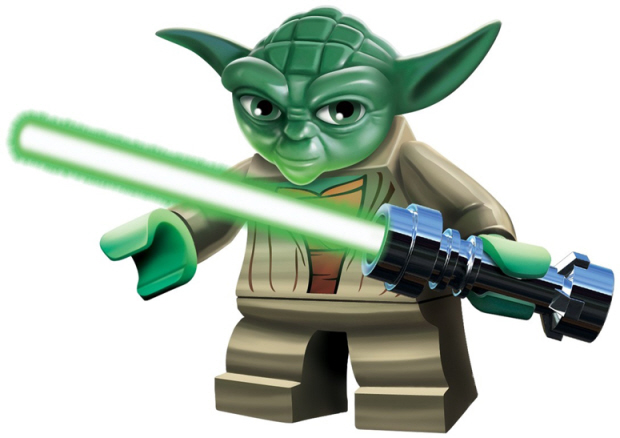
\includegraphics[width=0.8\textwidth]{Images/ImagenYoda.jpg}
    \label{fig:yoda}
\end{figure}

As\'i la Figura~\ref{fig:yoda} muestra una imagen que se encuentra en el directorio images, mientras la tabla~\ref{tab:tablasEx}, muestra dos ejemplos de información tabular con combinaci\'on de columnas, y combinaci\'on de filas.

\begin{table}[htbp!]
    \centering
    \caption{Ejemplo de tabla con multi columnas (arriba) y multi filas(abajo)}
    \begin{tabular}{ |p{3cm}||p{3cm}|p{3cm}|p{3cm}|  }
        \hline
        \multicolumn{4}{|c|}{Country List} \\
        \hline
        Country Name or Area Name& ISO ALPHA 2 Code &ISO ALPHA 3 Code&ISO numeric Code\\
        \hline
        Afghanistan   & AF    &AFG&   004\\
        Aland Islands&   AX  & ALA   &248\\
        Albania &AL & ALB&  008\\
        Algeria    &DZ & DZA&  012\\
        American Samoa&   AS  & ASM&016\\
        Andorra& AD  & AND   &020\\
        Angola& AO  & AGO&024\\
        \hline
    \end{tabular}\\
    \vspace{0.5cm}
    \begin{tabular}{ |c|c|c|c| } 
        \hline
        col1 & col2 & col3 \\
        \hline
        \multirow{3}{4em}{Multiple row} & cell2 & cell3 \\ 
        & cell5 & cell6 \\ 
        & cell8 & cell9 \\ 
        \hline
    \end{tabular}

    \label{tab:tablasEx}
\end{table}

Adem\'as se recomienda consultar los manuales que aparecen en al secci\'on de aprendizaje de overleaf, por ejemplo el de \href{https://www.overleaf.com/learn/latex/Tables}{tablas}.
    
    % Trabajos previos
    \chapter{Estado del Arte}
    % desarrollar el marco referencial el cual incluye, marco teórico, conceptual, histórico, referencial, científico, tecnológico entre otros.
% tratar de abordar la presentación de los marcos, a excepción del marco histórico, de lo general a lo específico

% Hay que contar como si fuera un cuento, en orden cronológico.

% Buscar cosas actuales de problemas similares
% Qué es lo más reciente y hacia a dónde se están dirigiendo las soluciones.


% Hay que contar la historia de lo que existe
% Desarrollar el estado del arte el cual debe incluir al menos uno de los siguientes marcos, teórico, conceptual, histórico, referencial, científico, tecnológico entre otros. Adem\'as se debe tratar de abordar la presentación de los marcos de lo general a lo específico, a excepción del marco histórico en donde se debe guardar un orden cronol\'ogico ascendente. 

\section*{Machine Learning en la Predicción de Precios Inmobiliarios}
El \textit{machine learning} (ML) es una rama de la inteligencia artificial que permite a las máquinas aprender de los datos y realizar predicciones sin necesidad de ser programadas explícitamente para cada tarea. En el contexto inmobiliario, los modelos de ML han demostrado ser particularmente útiles para predecir precios de propiedades, capturando patrones complejos en los datos que los métodos tradicionales no pueden detectar. Su aplicabilidad en el mercado inmobiliario surge de la capacidad de manejar grandes volúmenes de datos con múltiples variables, lo que mejora la precisión de las predicciones y facilita la toma de decisiones tanto para compradores como para inversionistas \cite{kim2018machinelearning}.

En Colombia, el mercado inmobiliario está influenciado por diversas características, como la ubicación geográfica, la seguridad y convivencia de las zonas, así como la cercanía a sitios de interés como centros comerciales y colegios. Con la disponibilidad de datos abiertos y técnicas de \textit{web scraping}, es posible recopilar información de diversas fuentes para enriquecer los modelos predictivos. Esta integración de características adicionales, como indicadores de seguridad, mapas de sitios cercanos, y boletines económicos, permite que los modelos de ML capturen mejor las relaciones no lineales y complejas entre los atributos de las viviendas y sus precios, como se observó en estudios previos \cite{zhang2018realestate}.

\subsection{Metodologías Tradicionales y su Limitación}
Los métodos hedónicos (tradicionales), ampliamente utilizados en estudios inmobiliarios, han sido la base para estimar precios a partir de características como el área, el número de habitaciones y la ubicación \cite{kim2018machinelearning}. Sin embargo, estos modelos lineales tienden a fallar cuando las relaciones entre las variables son no lineales o cuando intervienen factores externos complejos. Además, su desempeño depende en gran medida de la calidad y la disponibilidad de los datos.


\subsection*{Regresión Lineal}
La regresión lineal es uno de los métodos más simples y utilizados para la predicción de precios inmobiliarios. Este modelo asume una relación lineal entre las características de las propiedades (como área habitable, número de habitaciones, ubicación) y los precios. Aunque es un buen punto de partida, es limitado cuando las relaciones entre las variables no son lineales. En estudios como el de Kim et al. \cite{kim2018machinelearning}, se evidenció que la regresión lineal tiende a ser superada por modelos más complejos en mercados con dinámicas no lineales.

\textbf{Ventajas:} Simple de implementar y explicar.\\
\textbf{Desventajas:} No captura relaciones no lineales y es sensible a los \textit{outliers}.\\
\textbf{Casos de uso:} Predicción en mercados con relaciones lineales bien definidas.

\subsection*{Árboles de Decisión}
Los árboles de decisión son modelos no paramétricos que dividen los datos en subconjuntos más pequeños en función de las características más importantes. Este enfoque es especialmente útil cuando se desea interpretar los resultados, ya que los árboles permiten una visualización clara de cómo las características afectan el precio. Sin embargo, tienden a sobreajustarse a los datos de entrenamiento si no se controlan adecuadamente \cite{kim2018machinelearning}.

\textbf{Ventajas:} Fácil de interpretar y manejar datos con interacciones no lineales.\\
\textbf{Desventajas:} Propenso al sobreajuste, a menos que se utilicen técnicas de poda.\\
\textbf{Casos de uso:} Situaciones donde la interpretabilidad es importante y se requiere manejar relaciones no lineales.

\subsection*{Random Forest}
Random Forest es un algoritmo de aprendizaje conjunto que utiliza múltiples árboles de decisión para mejorar la precisión y reducir el riesgo de sobreajuste. Cada árbol se entrena en un subconjunto diferente de los datos, lo que reduce la variabilidad y mejora la generalización. En estudios como el de Zhang et al. \cite{zhang2018realestate}, Random Forest fue uno de los modelos más efectivos, debido a su capacidad para manejar un gran número de variables y sus interacciones.

\textbf{Ventajas:} Robusto frente al sobreajuste, puede manejar grandes conjuntos de datos y múltiples variables.\\
\textbf{Desventajas:} Menos interpretativo que un único árbol de decisión y requiere más recursos computacionales.\\
\textbf{Casos de uso:} Mercados inmobiliarios complejos con muchas características y donde las relaciones no son lineales.

\subsection*{XGBoost}
XGBoost es un algoritmo de \textit{boosting} que mejora iterativamente los errores de predicción de modelos más simples. En cada iteración, se construyen nuevos árboles que corrigen los errores de los árboles anteriores. Este modelo ha demostrado ser extremadamente eficaz en competiciones de predicción de precios debido a su alta precisión y velocidad. En estudios como el de Smith et al. \cite{bigdata2019realestate}, XGBoost mostró un rendimiento superior al de otros modelos de \textit{machine learning}, debido a su capacidad para manejar datos ruidosos y \textit{outliers}.

\textbf{Ventajas:} Alta precisión, robustez frente a datos ruidosos y capacidad para ajustar hiperparámetros de manera efectiva.\\
\textbf{Desventajas:} Requiere más tiempo de entrenamiento y ajuste de hiperparámetros.\\
\textbf{Casos de uso:} Situaciones donde se necesita maximizar la precisión de las predicciones en mercados inmobiliarios dinámicos y no lineales.

\subsection*{Redes Neuronales}
Las redes neuronales son modelos de \textit{machine learning} que se inspiran en la estructura del cerebro humano, lo que les permite aprender patrones complejos en los datos. Las redes neuronales profundas (\textit{deep learning}) son especialmente útiles cuando se manejan grandes volúmenes de datos con muchas variables. En estudios como el de Kim et al. \cite{kim2018machinelearning}, las redes neuronales demostraron ser efectivas en la captura de relaciones no lineales complejas, aunque requieren una gran cantidad de datos y recursos computacionales.

\textbf{Ventajas:} Captura relaciones no lineales complejas y se adapta bien a grandes volúmenes de datos.\\
\textbf{Desventajas:} Difícil de interpretar, requiere muchos datos y potencia computacional.\\
\textbf{Casos de uso:} Situaciones donde se dispone de grandes volúmenes de datos y la relación entre las características es altamente no lineal.

\subsection*{Comparación de Modelos}
Cada modelo tiene sus ventajas y limitaciones, por lo que la elección depende de las características del mercado inmobiliario en estudio. En el contexto colombiano, con la incorporación de variables adicionales como mapas de sitios de interés, proximidad a comercios y estaciones de transporte público, es probable que modelos como Random Forest y XGBoost, que pueden manejar relaciones complejas, resulten ser los más efectivos. Por otro lado, la regresión lineal puede ser útil en casos donde las relaciones entre variables son más simples.

La comparación de modelos en términos de precisión y eficiencia es esencial para seleccionar el enfoque más adecuado. Estudios previos han demostrado que los modelos de ensamble, como \textit{Random Forest} y \textit{Gradient Boosting}, ofrecen mejores resultados en la mayoría de los casos \cite{dabreo2021realestate, wang2019svr}. Adicionalmente, las redes neuronales profundas (\textit{Deep Learning}) han sido exploradas en escenarios donde se dispone de grandes volúmenes de datos \cite{mostofi2022realestate}.


\subsection{Aplicación de Machine Learning en la Predicción de Precios}
El uso de machine learning ha demostrado ser una alternativa efectiva a los métodos tradicionales. Modelos como \textit{Random Forest}, \textit{Gradient Boosting Machines (GBM)}, y \textit{Support Vector Machines (SVM)} han mostrado mejores resultados en la predicción de precios debido a su capacidad para manejar relaciones no lineales y variables complejas \cite{park2015housing, zhang2018realestate}. En particular, el modelo \textit{Gradient Boosting} se destacó por su precisión en varios estudios \cite{bigdata2019realestate}.

\subsection{Uso de Variables Externas en la Predicción de Precios}
Los factores externos, como la proximidad a centros comerciales, colegios y hospitales, y los índices de seguridad, son determinantes clave en los precios inmobiliarios. Estudios recientes han integrado estos factores en los modelos predictivos, mejorando significativamente su rendimiento \cite{li2017realestate, mostofi2022realestate}. Sin embargo, la mayoría de los trabajos se enfocan en mercados específicos, dejando un vacío en la generalización de estos enfoques a mercados emergentes como Bogotá.

\subsection{Desafíos y Oportunidades en la Predicción de Precios}
Entre los principales desafíos se encuentran la falta de datos completos y la dependencia de los modelos de machine learning en datos de alta calidad \cite{yu2016realestate}. Sin embargo, la integración de técnicas híbridas, como SVM optimizado por PSO (Particle Swarm Optimization), ofrece oportunidades para superar estas limitaciones \cite{zhang2018realestate}.

\subsection{Identificación de Brechas en la Literatura}
A pesar de los avances en la integración de variables externas, la mayoría de los estudios se han enfocado en mercados desarrollados, dejando un vacío en mercados emergentes como Bogotá. Este proyecto busca llenar esta brecha aplicando enfoques modernos a un contexto local y utilizando datos enriquecidos para mejorar la precisión de las predicciones.

\subsection{Conclusión}
El estado del arte demuestra que las técnicas de machine learning y el enriquecimiento de datos ofrecen una mejora significativa en la predicción de precios de bienes raíces. Sin embargo, existe una necesidad clara de explorar estos enfoques en mercados emergentes y evaluar el impacto de factores externos en los precios. Este proyecto se posiciona como una contribución relevante al abordar estas brechas y expandir las aplicaciones de machine learning en el sector inmobiliario.


    
    % Problema de investigacion
    \chapter{Problema de investigaci\'on}
    El déficit habitacional en Colombia, caracterizado por la falta de acceso a vivienda digna y equitativa, es una problemática compleja que afecta a millones de personas. Según Castillo (2004), el déficit habitacional en el país incluye tanto aspectos cuantitativos, como la insuficiencia de viviendas disponibles, como cualitativos, relacionados con la calidad de las viviendas y su entorno \cite{castillo2004anotaciones}. Este problema es especialmente agudo en Bogotá, donde el crecimiento desorganizado y la urbanización informal han exacerbado la marginalidad y la exclusión \cite{castillo2004anotaciones}.

Adicionalmente, el acceso limitado al financiamiento hipotecario y la especulación inmobiliaria contribuyen a distorsionar el mercado, encareciendo los precios y excluyendo a los hogares de bajos ingresos. Más del 80\% de los hogares de bajos ingresos no tiene acceso a créditos hipotecarios, lo que agrava la inequidad en el acceso a la vivienda \cite{castillo2004anotaciones}. Este panorama se ve reflejado en los cambios recientes en las políticas de subsidios, como \textit{Mi Casa Ya}, cuya implementación irregular ha afectado tanto a desarrolladores como a compradores, aumentando la incertidumbre en el sector \cite{coyunturaVivienda2023}.

En paralelo, la vivienda también ha sido utilizada históricamente como un instrumento de especulación financiera y política. La falta de integración de datos cualitativos, como la calidad de los servicios públicos, la accesibilidad y el equipamiento urbano, limita la capacidad de los modelos actuales de predicción de precios para reflejar las dinámicas reales del mercado. Los modelos tradicionales, basados únicamente en características extraídas de portales inmobiliarios, no consideran los factores sociales y económicos que afectan directamente los precios, como destacó Walter (2023) en su análisis de la desaceleración del sector vivienda en Colombia \cite{coyunturaVivienda2023, fortaleciendoVivienda2024}.

    
    % Justificación
    \chapter{Justificaci\'on}
    % describir brevemente que just¿ifica el desarrollo del proyecto de investigación

% incluir el alcance que tendrá el proyecto a desarrollar

La vivienda es un derecho fundamental reconocido en la Constitución de Colombia \cite{ConstitucionPoliticaColombia1991}, pero la inequidad en el acceso, el déficit habitacional y la especulación inmobiliaria muestran que este derecho no se garantiza de manera efectiva. Desarrollar un modelo predictivo robusto, que incorpore variables estructuradas y contextuales, podría ayudar a mitigar los problemas asociados al mercado inmobiliario. Este enfoque no solo permitiría mejorar las estimaciones de precios, sino también diseñar políticas públicas más efectivas y basadas en evidencia \cite{fortaleciendoVivienda2024, castillo2004anotaciones, coyunturaVivienda2023}.

La predicción precisa de precios de viviendas es un aspecto crucial en el mercado inmobiliario, no solo para compradores y vendedores, sino también para inversionistas, desarrolladores y gobiernos locales. Cuando las estimaciones de precios son imprecisas o están basadas en datos incompletos, se generan varios problemas que afectan tanto al mercado como a los actores involucrados.

\subsection*{Decisiones de compra y venta desinformadas}
Los propietarios que subestiman el valor de su vivienda pueden venderla por debajo de su verdadero precio de mercado, perdiendo oportunidades de obtener una mayor ganancia. Por otro lado, los compradores que reciben estimaciones infladas pueden adquirir propiedades por encima de su valor real, enfrentando dificultades para revenderlas o recuperar la inversión. Este fenómeno afecta directamente la equidad y la transparencia del mercado, creando desconfianza entre los participantes.

\subsection*{Desigualdad en la accesibilidad a la vivienda}
Cuando las estimaciones de precios no son precisas, las zonas de alto crecimiento pueden ser sobrevaloradas, y las de menor crecimiento pueden ser infravaloradas, lo que provoca una distorsión en la accesibilidad a la vivienda. Esto puede llevar a que sectores de la población, especialmente los de menores ingresos, sean excluidos de áreas en proceso de valorización, acelerando fenómenos de gentrificación y desplazamiento de comunidades.

\subsection*{Burbujas inmobiliarias y volatilidad en el mercado}
Las malas estimaciones de precios pueden contribuir a la formación de burbujas inmobiliarias, donde los precios se inflan artificialmente debido a una sobrevaloración de las propiedades. Cuando la burbuja estalla, los precios caen bruscamente, lo que provoca una crisis de confianza en el mercado y pérdidas económicas significativas para propietarios e inversionistas. Este tipo de volatilidad afecta la estabilidad financiera de las familias y las inversiones de largo plazo.

\subsection*{Dificultades para la planificación urbana}
Una buena estimación de precios es clave para la planificación urbana y la asignación de recursos en infraestructura, servicios públicos y desarrollo sostenible. Si las predicciones de precios no reflejan adecuadamente el valor futuro de las propiedades, los gobiernos locales y desarrolladores pueden tomar decisiones incorrectas sobre dónde invertir en infraestructura y servicios. Esto puede resultar en zonas sobrepobladas sin servicios adecuados o en áreas subdesarrolladas que no reciben suficiente inversión.

\subsection*{Pérdida de confianza de inversionistas}
Los inversionistas dependen de estimaciones precisas de precios para identificar oportunidades de crecimiento en diferentes zonas. Si los modelos utilizados no logran prever con exactitud la evolución de los precios, los inversionistas podrían enfrentar pérdidas o no alcanzar la rentabilidad esperada. Esto desalienta la inversión en el sector inmobiliario y puede impactar negativamente en el desarrollo económico local.

\subsection*{Impacto en el crédito hipotecario}
Las instituciones financieras basan sus decisiones de otorgamiento de crédito hipotecario en evaluaciones precisas del valor de las propiedades. Cuando estas evaluaciones están basadas en estimaciones incorrectas, el riesgo de impagos o de tener propiedades sobrevaluadas en el portafolio de préstamos aumenta. Esto puede derivar en pérdidas para los bancos y en restricciones más severas para otorgar créditos, afectando a las familias que buscan adquirir vivienda.

La correcta predicción de precios, basada en datos estructurados y enriquecidos, no solo mejorará la transparencia y eficiencia del mercado inmobiliario en Bogotá, sino que también evitará estos problemas derivados. Por lo tanto, el desarrollo de un modelo de predicción que incorpore tanto características internas de las propiedades como datos externos (seguridad, cercanía a servicios, etc.) podría ser fundamental para la sostenibilidad y el crecimiento del mercado inmobiliario, promoviendo una mayor equidad y una mejor toma de decisiones por parte de todos los actores involucrados.

    
    % Objetivos
    \chapter{Objetivos}
    % Incluye los objetivos general y específicos del proyecto. Debe procurar seguir una metodología de formulación de objetivos, por ejemplo S.M.A.R.T.

% Debe tener solo un verbo en infinitivo e incluír como lo van a medir a uno


\section{Objetivo general}

Desarrollar un modelo de predicción de precios de viviendas en Bogotá utilizando técnicas de \textit{machine learning}, que incorpore tanto características internas de las propiedades (como tamaño, número de habitaciones y ubicación) como datos externos (indicadores de seguridad, proximidad a puntos de interés, y accesibilidad a servicios), con el fin de mejorar la precisión en la estimación de precios y contribuir a la toma de decisiones informada en el mercado inmobiliario.


% Preprocesamiento
% Evitar modelos que se van a usar (modelos predictivos)
% No poner métricas

% General un modelo predictivo

\section{Objetivos específicos}
\begin{itemize}
    \item Crear una base de datos consolidada a partir de la recolección de información mediante \textit{web scraping} de diversas plataformas inmobiliarias en Bogotá.
    \item Enriquecer los datos obtenidos integrando información adicional proveniente de fuentes externas, como indicadores de seguridad, convivencia y proximidad a servicios.
    \item Seleccionar el mejor modelo de predicción de precios a partir de la comparación de un conjunto de modelos desarrollados, evaluando su rendimiento mediante métricas de precisión y eficiencia.
\end{itemize}


    
    % Metodologia
    \chapter{Metodolog\'ia de investigación}
    \section*{Metodología}
La metodología implementada comprende: (i) adquisición de datos base, (ii) limpieza y preprocesamiento con umbrales y reglas reproducibles, (iii) enriquecimiento geoespacial mediante capas del distrito y conteos de POIs (OSM), (iv) entrenamiento y evaluación de modelos base y aumentados, y (v) persistencia y exposición vía API.

\begin{figure}[h]
    \centering
    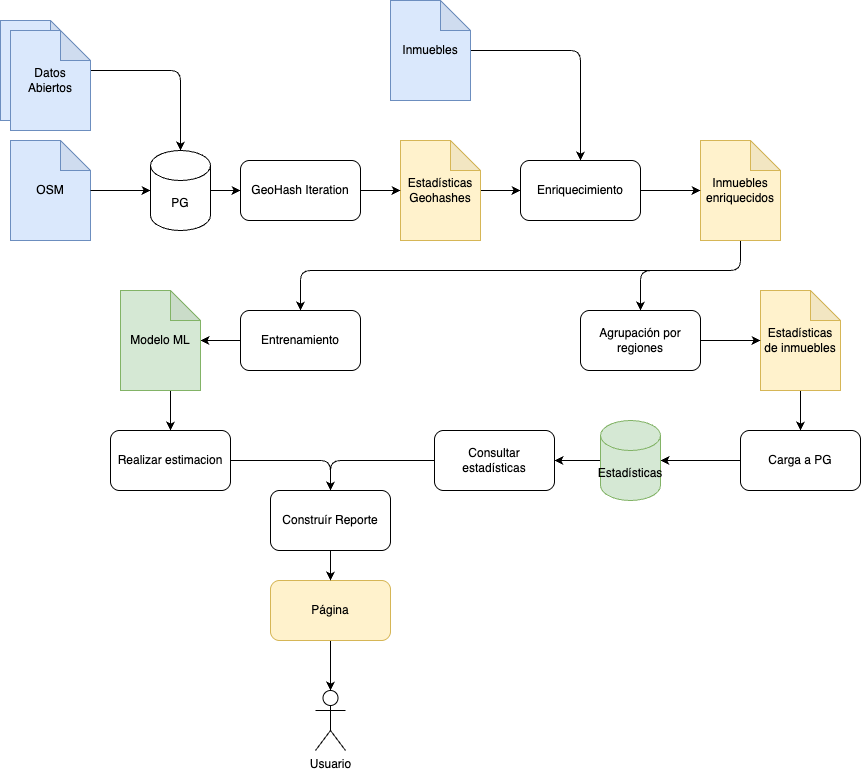
\includegraphics[width=0.85\linewidth]{Images/metodologia.png}
    \caption{Proceso general de la metodología}
    \label{fig:metodologia}
\end{figure}

\subsection*{Fuentes de datos}
\begin{itemize}
    \item \textbf{Datos de inmuebles (base)}: JSON único de agosto de 2024 publicado en GitHub (\texttt{builker-col/bogota-apartments}). Se procesó a CSV.
    \item \textbf{Datos abiertos del distrito (PostGIS)}: capas consultadas en agosto de 2025: \texttt{barrios\_bogota}, \texttt{upz\_bogota}, \texttt{localidades\_bogota}, \texttt{estratos\_manzana}, \texttt{avaluo\_catastral\_manzana}, y POIs OSM (\texttt{gis\_osm\_pois\_free\_1}, \texttt{gis\_osm\_pois\_a\_free\_1}), con SRID esperado 4326 \cite{datosabiertos_bogota}.
\end{itemize}

\subsection*{Limpieza y preprocesamiento}
Realizado en Python (\textit{Pandas}, \textit{NumPy}, \textit{scikit-learn}) sobre el CSV base:
\begin{itemize}
    \item \textbf{Outliers}: filtro por percentil 99. \emph{Área} \(\leq 464\,m^2\), \emph{precio\_venta} \(\leq 5{,}4\times 10^9\) COP.
    \item \textbf{Precio mínimo}: \(\geq 50{,}000{,}000\) COP.
    \item \textbf{Área igual a 0}: imputación por mediana de comparables (mismo \emph{estrato}, \emph{habitaciones}, \emph{banos}, \emph{sector}); si no hay, mediana por \emph{estrato}.
    \item \textbf{Parqueaderos negativos}: reemplazo por moda dentro del mismo \emph{estrato} (sino, moda global).
    \item \textbf{Coordenadas}: imputación por mediana del \emph{sector} o global cuando estén fuera de Bogotá; bounding box final: lat \([4.4, 4.9]\), lon \([-74.3, -73.9]\). Registros fuera se eliminan tras imputación.
    \item \textbf{Estrato fuera de rango [1--6]}: imputación por modo del \emph{sector}; si no hay, modo global.
\end{itemize}

\subsection*{Enriquecimiento geoespacial}
Se calcula por propiedad (lat, lon) con un pipeline asíncrono y persistencia en PostGIS:
\begin{itemize}
    \item \textbf{Conteos de POIs OSM} por radios de 100, 300, 500, 1000 y 2000 metros en categorías agregadas: \emph{education}, \emph{healthcare}, \emph{retail\_access}, \emph{dining\_and\_entertainment}, \emph{accommodation}, \emph{parks\_and\_recreation}, \emph{infrastructure\_services}, \emph{cultural\_amenities}.
    \item \textbf{Metadatos regionales}: asignación de UPZ, barrio y localidad; variables \emph{upz\_calculada}, \emph{barrio\_calculado}, \emph{localidad\_calculada}.
    \item \textbf{Valuación por geohash}: promedios de \emph{catastral} y \emph{comercial} por celda (geohash), usando \texttt{avaluo\_catastral\_manzana}.
    \item \textbf{Persistencia y estadísticas}: escritura en \texttt{property\_data} y agregación en \texttt{region\_stats} (barrio, UPZ, localidad) vía \texttt{ST\_Contains}, con \(n\), medias, desviaciones y cuartiles.
\end{itemize}

\subsection*{Modelos base}
Conjunto de modelos evaluados con validación cruzada \(KFold=5,\ \texttt{shuffle=True},\ \texttt{random\_state=42}\), métrica RMSE (escala real). Preprocesamiento: \texttt{SimpleImputer} (media/moda), \texttt{StandardScaler}, \texttt{OneHotEncoder}. Resultados (aprox.):
\begin{itemize}
    \item \textbf{Random Forest}: RMSE \(\approx\) 245M (CV); en\ hold-out (20\%): RMSE \(\approx\) 250.6M, MAE \(\approx\) 129.9M, R\textsuperscript{2} \(\approx\) 0.915.
    \item \textbf{XGBoost / LightGBM}: RMSE \(\approx\) 245--246M (CV).
    \item \textbf{Lineales}: \(\approx\) 348M; \textbf{SVR}: \(\approx\) 913M.
\end{itemize}
Se evaluó además con \(\log(\textit{precio\_venta})\) y \(\log(\textit{area})\), mejorando métricas en escala original.

\subsection*{Modelos con datos aumentados}
Se entrenaron variantes con variables enriquecidas y selección reducida:
\begin{itemize}
    \item \textbf{v0 (XGB)}: \(\log(\textit{area})\), one-hot; variables estructurales dominan; enriquecidas con aporte marginal.
    \item \textbf{v1 (XGB reducido + barrio\_top)}: hold-out RMSE \(\approx\) 254.66M, MAE \(\approx\) 136.54M, R\textsuperscript{2} \(\approx\) 0.9139. Modelo exportado como \texttt{xgboost\_model\_2.1.pkl}.
    \item \textbf{v2 (XGB con búsqueda aleatoria)}: mejores hiperparámetros: \(n\_\textit{estimators}=500\), \(\textit{max\_depth}=9\), \(\textit{learning\_rate}=0.05\), \(\textit{subsample}=0.8\), \(\textit{colsample\_bytree}=0.8\), \(\alpha=0\), \(\lambda=1\). Hold-out: RMSE \(\approx\) 233.49M, MAE \(\approx\) 121.96M, R\textsuperscript{2} \(\approx\) 0.9276. Exportado como \texttt{xgboost\_model\_2.2.pkl}.
\end{itemize}

\subsection*{Exposición de resultados y API}
Se expone un endpoint \texttt{GET /api/estimate} (FastAPI) que combina estadísticas del punto (POIs, región, valuación) y la predicción del modelo: agrega \texttt{get\_point\_stats}, \texttt{get\_region\_stats} y \texttt{estimate(...)} sobre la versión de modelo configurada (por defecto 2.1; se recomienda 2.2 por mejor RMSE).

\subsection*{Reproducibilidad}
Los notebooks en \texttt{analisis/notebooks/} contienen el detalle de extracción, limpieza, evaluación y entrenamiento; el proyecto \texttt{indexador-py/} encapsula el enriquecimiento y la persistencia en PostGIS. Se controlaron semillas aleatorias y configuración de validación para permitir replicación de métricas.


    
    % Cronograma
    \chapter{Resultados y An\'alisis}
    \section{Resultados}
\subsection{Modelo base}
Se evaluaron múltiples algoritmos con validación cruzada (KFold=5, \texttt{shuffle=True}, \texttt{random\_state=42}), usando RMSE en escala real. El mejor desempeño base lo obtuvo \textbf{Random Forest}:
\begin{itemize}
    \item \textbf{CV (aprox)}: RF \(\approx\) 245M; XGB \(\approx\) 245M; LGBM \(\approx\) 246M; lineales \(\approx\) 348M; SVR \(\approx\) 913M.
    \item \textbf{Hold-out (20\%)}: RF RMSE \(\approx\) 250.6M; MAE \(\approx\) 129.9M; R\textsuperscript{2} \(\approx\) 0.915.
\end{itemize}
El uso de transformaciones \(\log(\textit{precio\_venta})\) y \(\log(\textit{area})\) mejoró las métricas al regresar a la escala original.

\subsection{Modelos con datos aumentados}
Tras enriquecer con variables contextuales (POIs por radio, asignación de UPZ/barrio/localidad, avalúos por geohash) se entrenaron variantes XGBoost:
\begin{itemize}
    \item \textbf{v1 (reducido + \textit{barrio\_top})}: RMSE \(\approx\) 254.66M; MAE \(\approx\) 136.54M; R\textsuperscript{2} \(\approx\) 0.9139. Modelo exportado: \texttt{xgboost\_model\_2.1.pkl}.
    \item \textbf{v2 (búsqueda aleatoria)}: hiperparámetros: \(n\_\textit{estimators}=500\), \(\textit{max\_depth}=9\), \(\textit{learning\_rate}=0.05\), \(\textit{subsample}=0.8\), \(\textit{colsample\_bytree}=0.8\), \(\alpha=0\), \(\lambda=1\). Hold-out: RMSE \(\approx\) 233.49M; MAE \(\approx\) 121.96M; R\textsuperscript{2} \(\approx\) 0.9276. Modelo exportado: \texttt{xgboost\_model\_2.2.pkl}.
\end{itemize}

\subsection{Importancia de variables y hallazgos}
\begin{itemize}
    \item \textbf{Variables dominantes}: \emph{área}, \emph{latitud}, \emph{administración}, \emph{antigüedad}, \emph{longitud} aparecen consistentemente entre las más relevantes.
    \item \textbf{Contexto espacial}: las variables de POIs por radio aportan de forma complementaria; su efecto es menor que el de las estructurales pero mejora el ajuste en v2.
    \item \textbf{Distribución del error}: el percentil 80 del error absoluto se ubica en torno a \(\sim\)187M para el RF base; v2 reduce RMSE y MAE manteniendo estabilidad.
\end{itemize}

\subsection{Artefactos y reproducibilidad}
\begin{itemize}
    \item Modelos serializados en \texttt{analisis/data/models/}: \texttt{randomforest\_model\_base.pkl}, \texttt{xgboost\_model\_2.1.pkl}, \texttt{xgboost\_model\_2.2.pkl}.
    \item Dataset enriquecido: \texttt{analisis/data/aptos\_bogota\_enriched.csv}.
    \item Pipeline de estimación expuesto vía \texttt{GET /api/estimate} en el backend (ver metodología).
\end{itemize}


    
    % Presupuesto
    \chapter{Discusi\'on}
    % Incluir el presupuesto necesario para el desarrollo del proyecto, estime los recursos necesarios y el costo de cada uno de ellos así como el de cada una de las horas del trabajo de los involucrados en el desarrollo del proyecto

% Incluir el presupuesto necesario para el desarrollo del proyecto, estime los recursos necesarios y el costo de cada uno de ellos así como el de cada una de las horas del trabajo de los involucrados en el desarrollo del proyecto, a continuaci\'on se provee un ejemplo del presupuesto

Se ha realizado una estimación de costos para el procesamiento de datos de Global Fishing Watch utilizando Amazon SageMaker, considerando un tamaño de dataset de 10 GB, el uso de instancias de tipo \texttt{ml.m5.large} para procesamiento y entrenamiento, y almacenamiento en Amazon S3. El procesamiento se estima en 8 horas diarias durante 20 días al mes, con 5 modelos entrenados al mes, cada uno tomando 10 horas. Los costos mensuales incluyen \$18.56 para procesamiento, \$5.80 para entrenamiento y \$0.23 para almacenamiento, resultando en un costo total mensual de \$24.59. Para un periodo de 15 meses (abril 2024 - junio 2025), el costo total estimado es de aproximadamente \$368.85.

\section{Tabla de Estimación de Costos}

\begin{table}[h!]
\centering
\caption{Estimación de costos para el procesamiento de datos de Global Fishing Watch usando Amazon SageMaker}
\begin{tabular}{|m{6cm}|m{4cm}|m{4cm}|}
\hline
\textbf{Concepto} & \textbf{Costo Mensual (\$)} & \textbf{Total para 15 meses (\$)} \\
\hline
Procesamiento (SageMaker) & 18.56 & 278.40 \\
\hline
Entrenamiento de Modelos & 5.80 & 87.00 \\
\hline
Almacenamiento (S3) & 0.23 & 3.45 \\
\hline
\textbf{Costo Total} & \textbf{24.59} & \textbf{368.85} \\
\hline
\end{tabular}
\end{table}


    
    % Resultados esperados
    \chapter{Conclusiones y Trabajo Futuro}
    
% Incluya los resultados esperados del desarrollo del proyecto de investigación en el marco del programa de Maestría en Inteligencia Artificial desde tres perspectivas: 

\begin{table}[htbp!]
    \centering
    \caption{Resultados o productos esperados de nuevo conocimiento.}
    \pgfplotstabletypeset[
	  col sep=colon, 
	  trim cells=true,
	  column type={|p{0.30\textwidth}|p{0.40\textwidth}|p{0.30\textwidth}}, 
	  columns/Resultado/.style = {column name={\cellcolor{AzulInstitucional}\textbf{\color{Blanco}Resultado o Producto esperado}}}, 
	  columns/Indicador/.style = {column name={\cellcolor{AzulInstitucional}\textbf{\color{Blanco}Indicador }}},
	  columns/Beneficiario/.style = {column name={\cellcolor{AzulInstitucional}\textbf{\color{Blanco}Beneficiario}}},
	  every head row = { \hline},
	  after row = {\hline},
	  string type,
	  skip rows between index={10}{20}
	]
	{Tables/DataNuevoConocimiento.csv}
    \label{tab:resEspNuecoConocimiento}
\end{table}


La anterior tabla resume los resultados esperados del actual proyecto desde tres perspectivas clave:

\begin{enumerate}
    \item Generación de nuevo conocimiento
    \item Fortalecimiento de la capacidad científica nacional
    \item Apropiación social del conocimiento
\end{enumerate}

Cada resultado esperado se acompaña de indicadores específicos para medir su éxito y los beneficiarios principales que se verán impactados positivamente por el proyecto.

% A continuaci\'on se presenta una tablas para la consolidaci\'on de estos resultados esperados a manera de ejemplo.





    
    % Anexos
    \chapter*{Anexos}
    % \section{Manual de instalación}

% \section{Manual de usuario}

% \section{Informe de ejecución de pruebas}

\section{Anexo técnico}

\subsection{Capas PostGIS y SRID}
\begin{itemize}
    \item \textbf{Capas}: \texttt{barrios\_bogota}, \texttt{upz\_bogota}, \texttt{localidades\_bogota}, \texttt{estratos\_manzana}, \texttt{avaluo\_catastral\_manzana}, \texttt{gis\_osm\_pois\_free\_1}, \texttt{gis\_osm\_pois\_a\_free\_1} \cite{datosabiertos_bogota}.
    \item \textbf{SRID}: 4326 (WGS84). Para consultas por distancia se usa proyección a 3857 cuando aplica (\texttt{ST\_Transform}).
    \item \textbf{Consultas típicas}: \texttt{ST\_DWithin}, \texttt{ST\_Contains}, \texttt{ST\_Intersects}, centroids y buffers en metros.
\end{itemize}

\subsection{Sistemas de referencia: WGS84 (EPSG:4326) y Web Mercator (EPSG:3857)}\label{annex:crs}
\begin{itemize}
    \item \textbf{WGS84 (EPSG:4326)}: sistema geodésico global usado por GPS. \emph{Coordenadas en grados} (latitud/longitud). Ventaja: interoperabilidad y exactitud posicional. Limitación: los grados no son métricos; 1$^{\circ}$ de longitud equivale a distintas distancias según la latitud.
    \item \textbf{Web Mercator (EPSG:3857)}: proyección métrica popular para mapas web. \emph{Coordenadas en metros} (pseudo-mercator). Ventaja: permite cálculos de distancia y \texttt{ST\_DWithin} en \emph{metros}. Limitación: distorsiona áreas y distancias al alejarse del ecuador (aceptable para escalas urbanas como Bogotá).
    \item \textbf{Cuándo usar cada uno}: almacenar y cruzar capas administrativas en 4326; proyectar a 3857 para consultas con radios en metros o buffers métricos (\texttt{ST\_Transform(geom, 3857)}).
    \item \textbf{Implicaciones en PostGIS}: para \texttt{ST\_DWithin} con radio en metros, asegure que ambas geometrías estén en 3857; para \texttt{ST\_Contains}/\texttt{ST\_Intersects} topológicos, 4326 es suficiente.
\end{itemize}

\subsection{Reglas de limpieza}
\begin{itemize}
    \item \textbf{Outliers (p99)}: \emph{área} \(\leq 464\,m^2\), \emph{precio\_venta} \(\leq 5{,}4\times10^9\) COP.
    \item \textbf{Precio mínimo}: \(\geq 50{,}000{,}000\) COP.
    \item \textbf{Área = 0}: mediana de comparables (\emph{estrato}, \emph{habitaciones}, \emph{banos}, \emph{sector}); si no hay, mediana por \emph{estrato}.
    \item \textbf{Parqueaderos < 0}: reemplazo por moda del mismo \emph{estrato}; si no hay, moda global.
    \item \textbf{Coordenadas}: imputación por mediana del \emph{sector} y filtro final a Bogotá: lat \([4.4,4.9]\), lon \([-74.3,-73.9]\).
    \item \textbf{Estrato fuera [1--6]}: imputación por modo del \emph{sector}; si no hay, modo global.
\end{itemize}

\subsection{Enriquecimiento geoespacial}
\begin{itemize}
    \item \textbf{Conteos OSM por radio}: 100, 300, 500, 1000, 2000 m.
    \item \textbf{Categorías}: \emph{education}, \emph{healthcare}, \emph{retail\_access}, \emph{dining\_and\_entertainment}, \emph{accommodation}, \emph{parks\_and\_recreation}, \emph{infrastructure\_services}, \emph{cultural\_amenities}.
    \item \textbf{Región calculada}: \emph{upz\_calculada}, \emph{barrio\_calculado}, \emph{localidad\_calculada} por \texttt{ST\_Contains}.
    \item \textbf{Avalúos por geohash}: promedios de \emph{catastral} y \emph{comercial} en bbox del geohash sobre \texttt{avaluo\_catastral\_manzana}.
    \item \textbf{Persistencia}: tabla \texttt{property\_data} adaptada al DF y agregados \texttt{region\_stats} (barrio/UPZ/localidad) con \(n\), medias, desviaciones y cuartiles.
\end{itemize}

\subsection{Modelos, métricas e hiperparámetros}
\begin{itemize}
    \item \textbf{Validación}: KFold=5 (\texttt{shuffle=True}, \texttt{random\_state=42}); métrica principal RMSE (escala real).
    \item \textbf{Base}: RF \(\approx\) 245M (CV); hold-out (20\%): RMSE \(\approx\) 250.6M, MAE \(\approx\) 129.9M, R\textsuperscript{2} \(\approx\) 0.915.
    \item \textbf{Aumentados}: v1 (XGB reducido + \emph{barrio\_top}) RMSE \(\approx\) 254.66M; v2 (XGB tuning) RMSE \(\approx\) 233.49M.
    \item \textbf{Hiperparámetros v2}: \(n\_\textit{estimators}=500\), \(\textit{max\_depth}=9\), \(\textit{learning\_rate}=0.05\), \(\textit{subsample}=0.8\), \(\textit{colsample\_bytree}=0.8\), \(\alpha=0\), \(\lambda=1\).
\end{itemize}

\subsection{API y operación}
\begin{itemize}
    \item \textbf{Endpoint}: \texttt{GET /api/estimate} (FastAPI). Entrada: lat, lon y atributos de la propiedad; salida: estadísticos del punto/region y predicción del modelo.
    \item \textbf{Modelo por defecto}: 2.1 (recomendado 2.2 por menor RMSE).
    \item \textbf{Ambiente}: PostGIS con SRID 4326; consultas en metros usando \texttt{ST\_Transform} a 3857.
\end{itemize}

\subsection{Reproducibilidad}
\begin{itemize}
    \item Notebooks en \texttt{analisis/notebooks/} para descarga, limpieza, EDA y entrenamiento.
    \item Artefactos de modelos en \texttt{analisis/data/models/} (\texttt{randomforest\_model\_base.pkl}, \texttt{xgboost\_model\_2.1.pkl}, \texttt{xgboost\_model\_2.2.pkl}).
    \item Enriquecimiento y persistencia en \texttt{indexador-py/} (ETL asíncrono, inserción por lotes, creación dinámica de tabla).
    \item Semillas y configuración de validación fijadas para replicar métricas.
\end{itemize}


    
    % Indices
    % \chapter*{\'Indices}
    % \input{BackMatter/B10-Index}
    
	% Incluye las referencias
    \bibliographystyle{apalike}
    \bibliography{Bibliography/referencias}

\end{document}
